\section{Additional Experimental Results}
\begin{figure}
     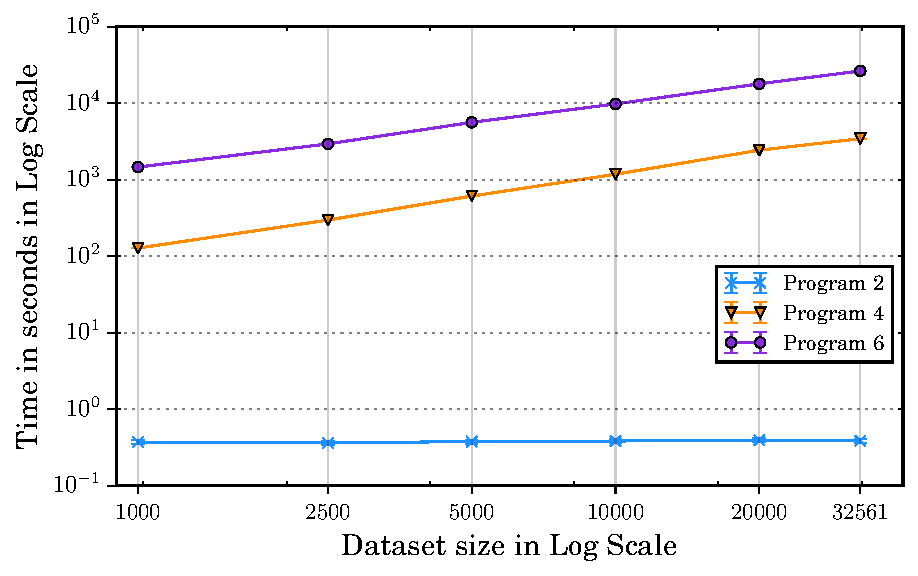
\includegraphics[width=0.5\linewidth]{scale2.pdf}
        \caption{Scalability of \system Programs Cntd.}\label{scale}
    \end{figure}
    \begin{figure}
     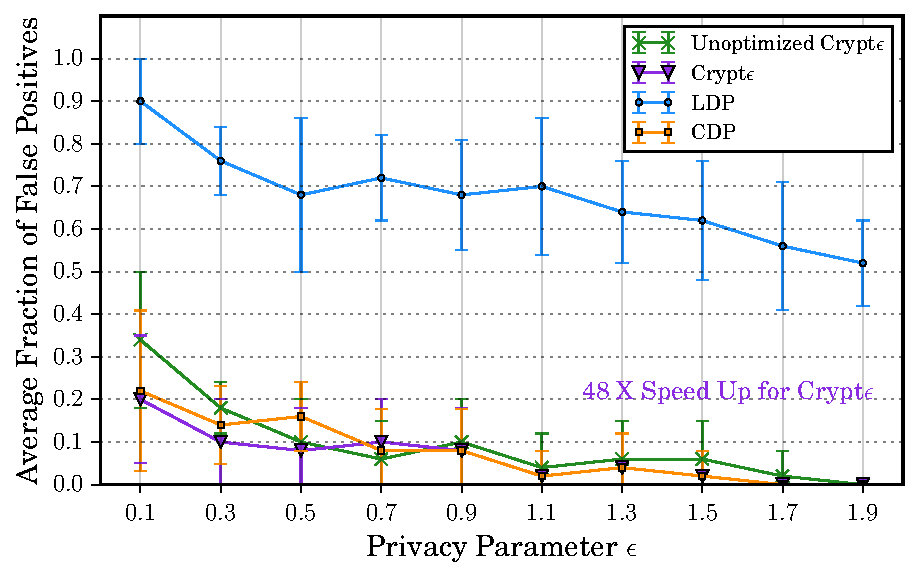
\includegraphics[width=0.5\linewidth]{2_final.pdf}
        \caption{Accuracy Analysis of \system Program 2 }\label{scale}
    \end{figure}
    \begin{figure}
     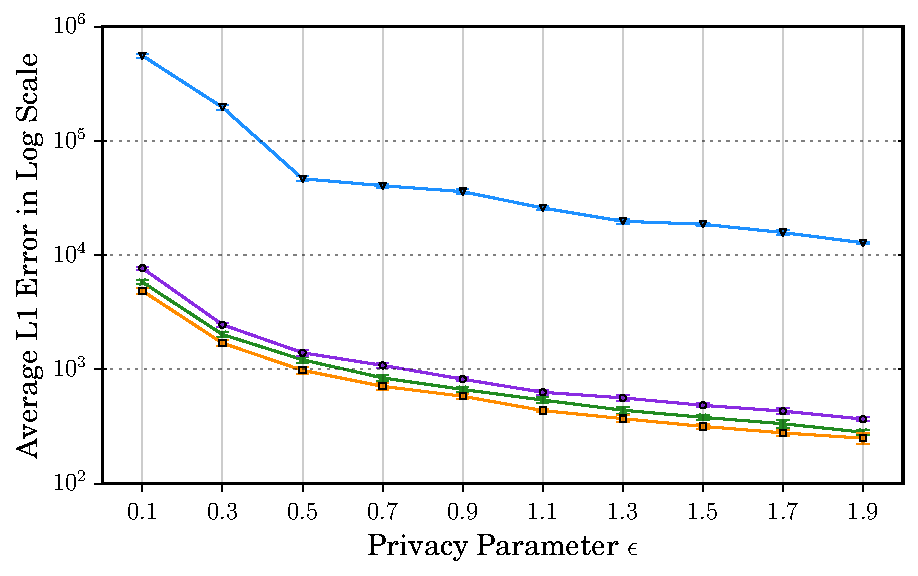
\includegraphics[width=0.5\linewidth]{4_final.pdf}
        \caption{Accuracy Analysis of \system Program 4 }\label{scale}
    \end{figure}
    \begin{figure}
     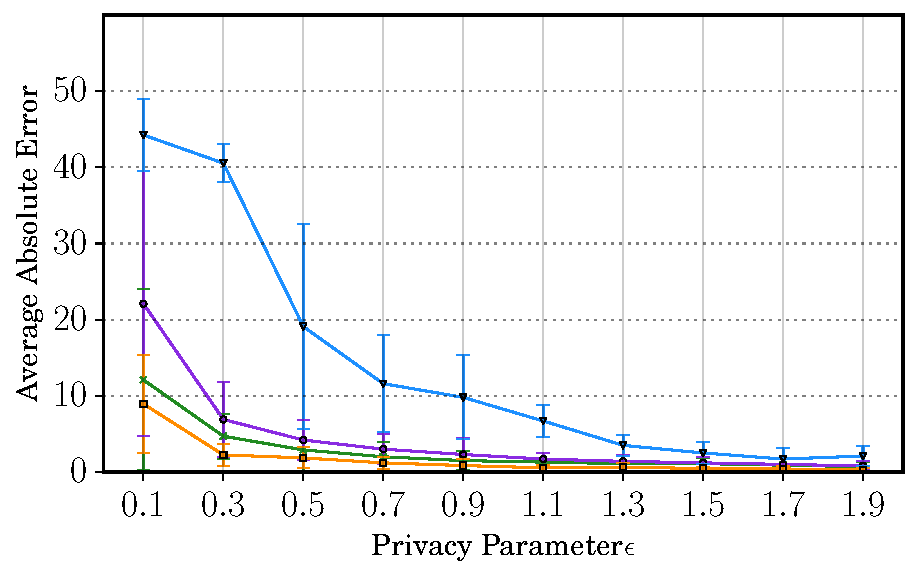
\includegraphics[width=0.5\linewidth]{6_finals.pdf}
        \caption{Accuracy Analysis of \system Program 6 }\label{scale}
    \end{figure}
\eat{\begin{figure*}
    \begin{subfigure}[b]{0.25\linewidth}
        \centering
        %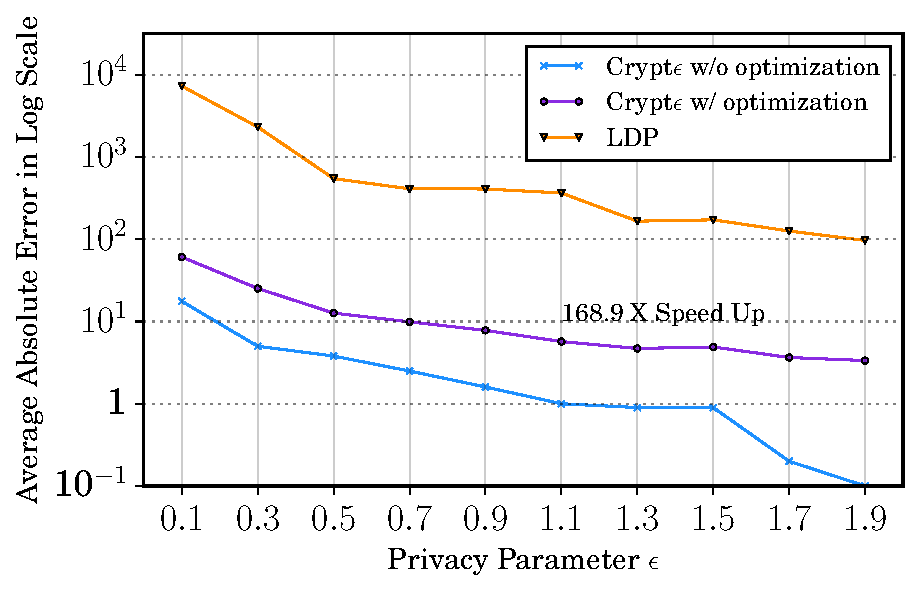
\includegraphics[width=5cm,height=3.1cm]{t1.pdf}
         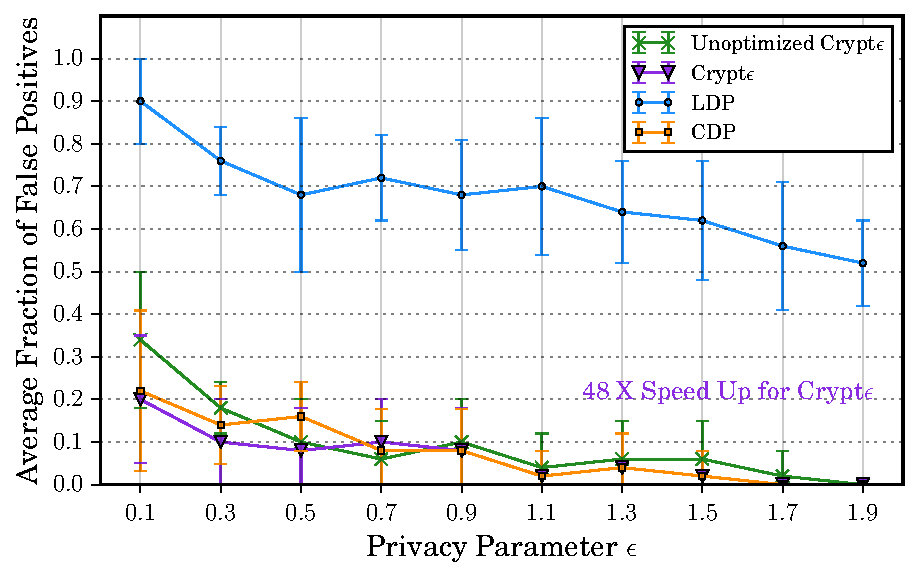
\includegraphics[width=1\linewidth]{2_final.pdf}
        \caption{ Program 2}
        \label{fig:P2}
    \end{subfigure}
    \begin{subfigure}[b]{0.25\linewidth}
    \centering 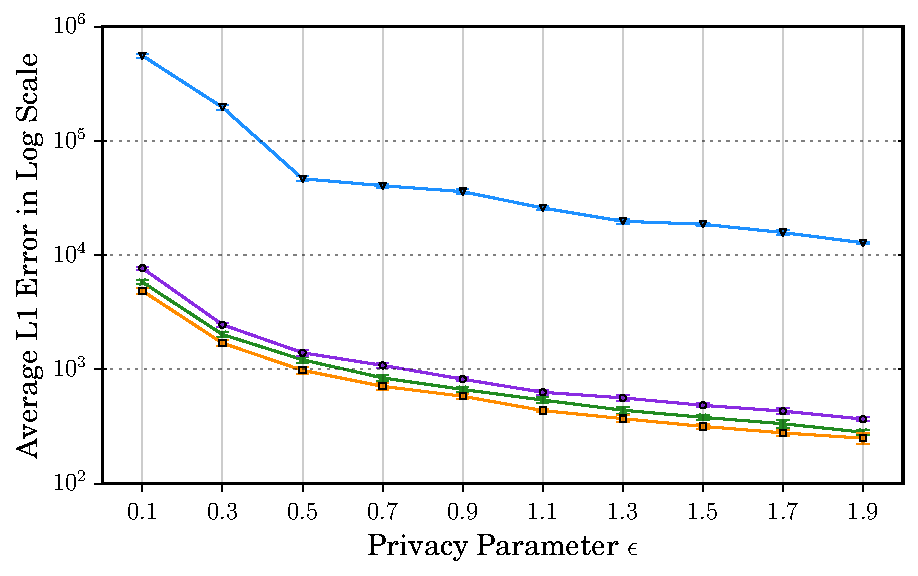
\includegraphics[width=1\linewidth]{4_final.pdf}
        \caption{Program 4}
        \label{fig:P4}\end{subfigure}
    \begin{subfigure}[b]{0.25\linewidth}
    \centering    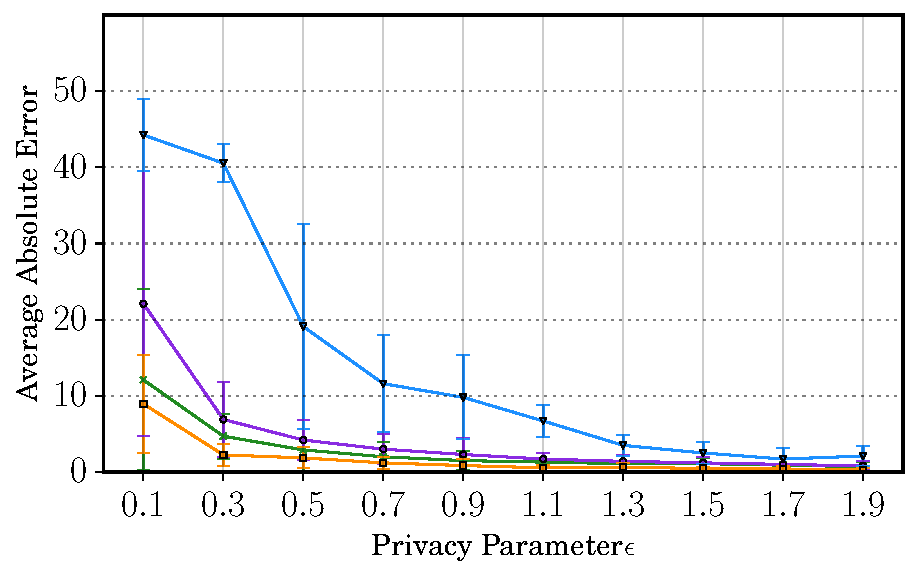
\includegraphics[width=1\linewidth]{6_finals.pdf}
        \caption{Program 6}
        \label{fig:P6}\end{subfigure}
   \caption{Accuracy Analysis of Crypt$\epsilon$ Programs Cntd.}
   \label{accuracy}
\end{figure*}

 
\stitle{Metrics:}\\
\textit{Accuracy}}

